\documentclass{standalone}
\usepackage{tikz}
\usetikzlibrary{patterns, positioning}
\usepackage[sfdefault]{ClearSans} %% option 'sfdefault' activates Clear Sans as the default text font
\usepackage[T1]{fontenc}

\begin{document}
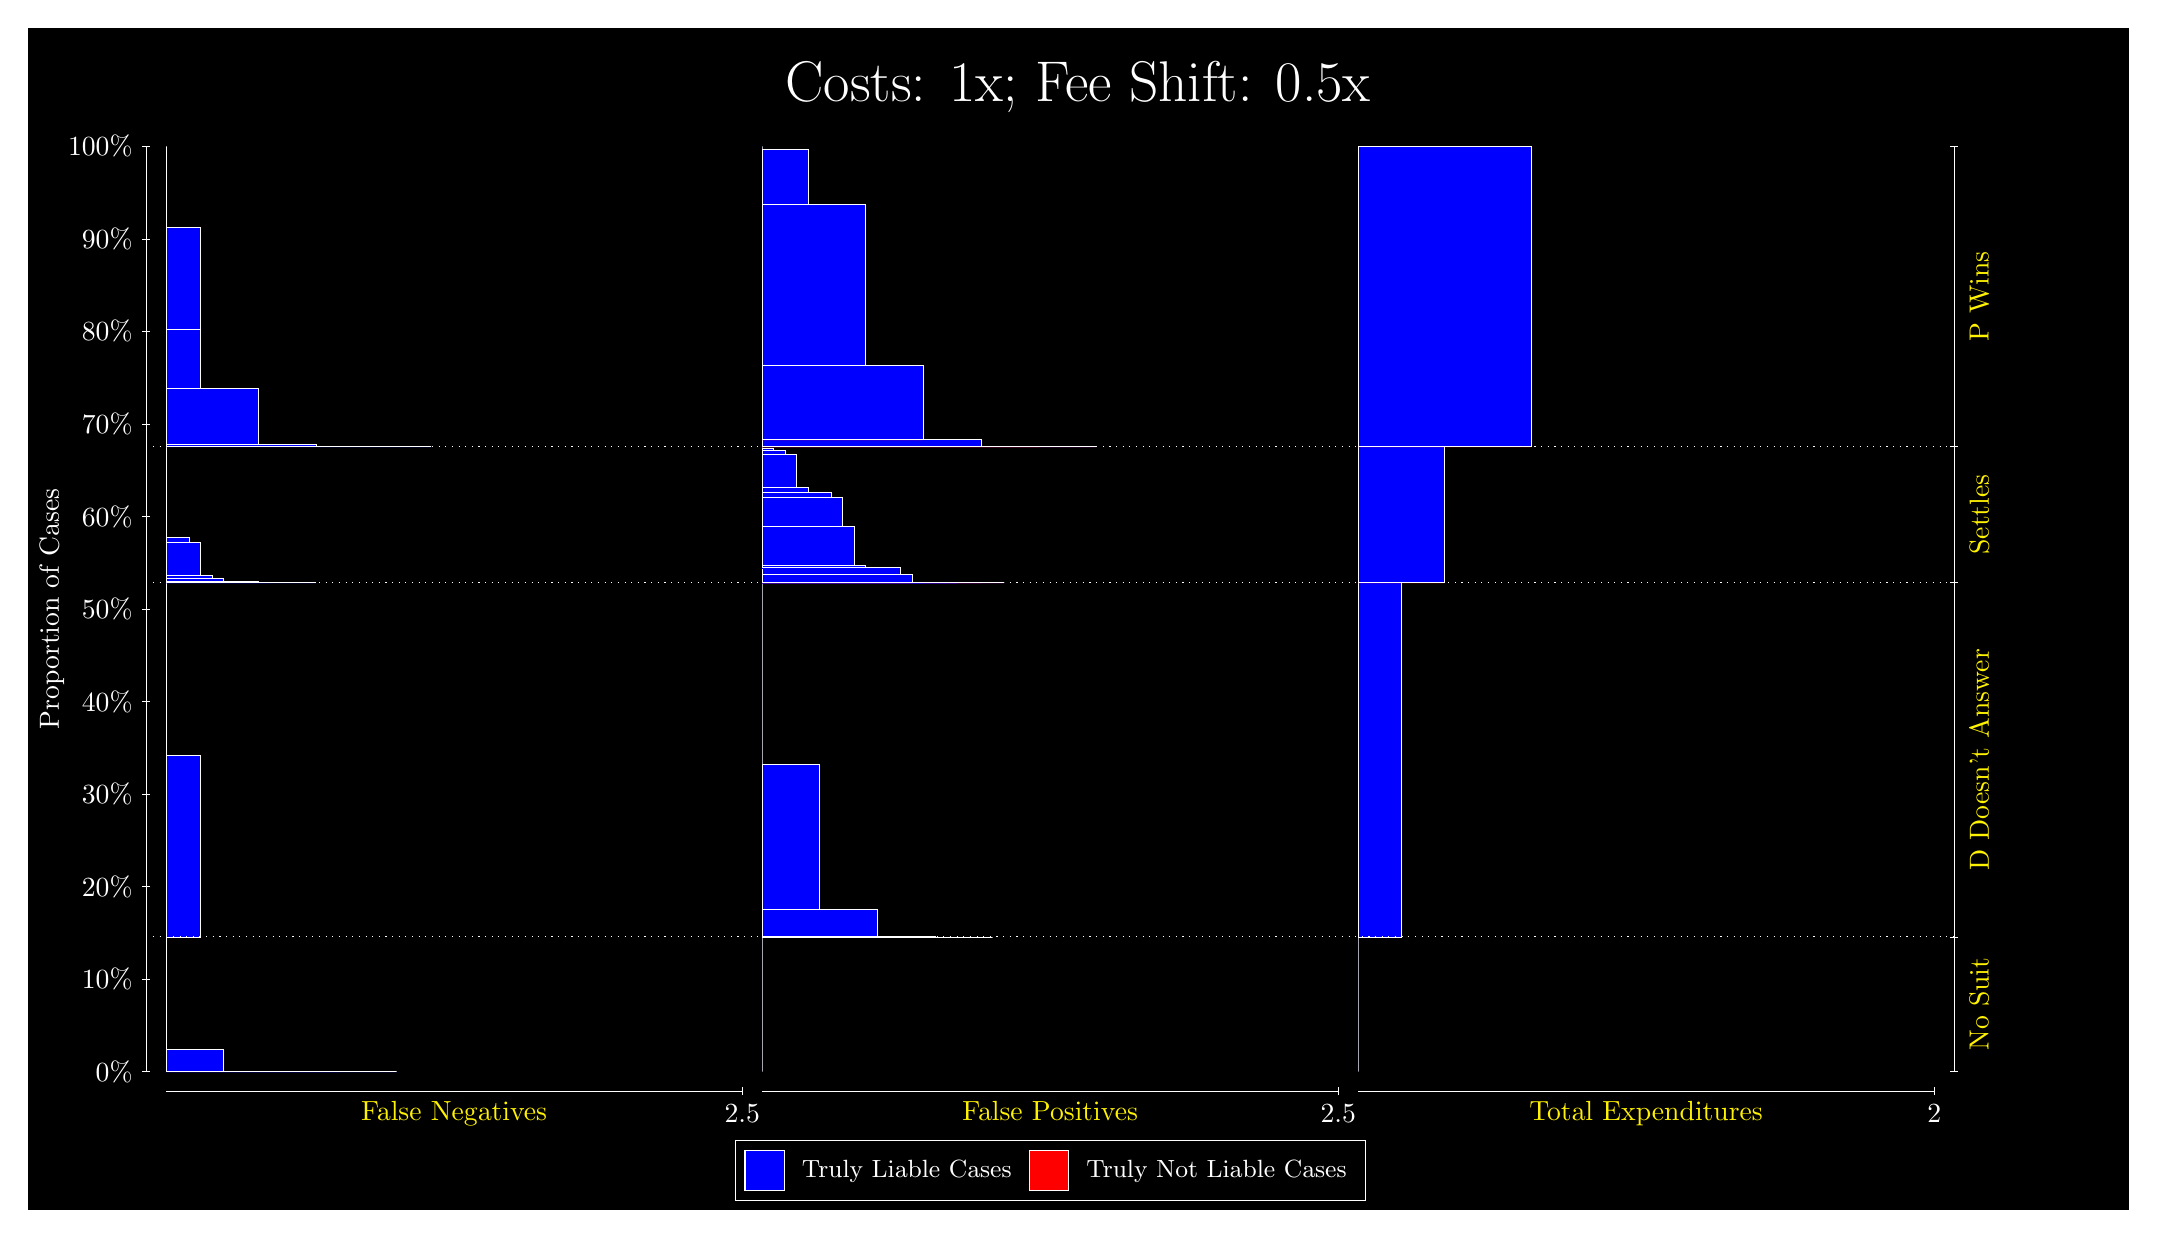
\begin{tikzpicture}
\draw[fill=black] (0,0) rectangle (26.667,15);
\draw[text=white] (0,13.5) rectangle (26.667,15) node[midway] {\huge Costs: 1x; Fee Shift: 0.5x};
\draw[white, very thin] (1.5,1.75) -- (1.5,13.5);
\node[rotate=90, text=white, anchor=center] at (0.3, 7.625) {Proportion of Cases};
\draw[white, very thin] (1.45,1.75) -- (1.55,1.75);
\node[text=white, anchor=east] at (1.45, 1.75) {0\%};
\draw[white, very thin] (1.45,2.925) -- (1.55,2.925);
\node[text=white, anchor=east] at (1.45, 2.925) {10\%};
\draw[white, very thin] (1.45,4.1) -- (1.55,4.1);
\node[text=white, anchor=east] at (1.45, 4.1) {20\%};
\draw[white, very thin] (1.45,5.275) -- (1.55,5.275);
\node[text=white, anchor=east] at (1.45, 5.275) {30\%};
\draw[white, very thin] (1.45,6.45) -- (1.55,6.45);
\node[text=white, anchor=east] at (1.45, 6.45) {40\%};
\draw[white, very thin] (1.45,7.625) -- (1.55,7.625);
\node[text=white, anchor=east] at (1.45, 7.625) {50\%};
\draw[white, very thin] (1.45,8.8) -- (1.55,8.8);
\node[text=white, anchor=east] at (1.45, 8.8) {60\%};
\draw[white, very thin] (1.45,9.975) -- (1.55,9.975);
\node[text=white, anchor=east] at (1.45, 9.975) {70\%};
\draw[white, very thin] (1.45,11.15) -- (1.55,11.15);
\node[text=white, anchor=east] at (1.45, 11.15) {80\%};
\draw[white, very thin] (1.45,12.325) -- (1.55,12.325);
\node[text=white, anchor=east] at (1.45, 12.325) {90\%};
\draw[white, very thin] (1.45,13.5) -- (1.55,13.5);
\node[text=white, anchor=east] at (1.45, 13.5) {100\%};

\draw[white, very thin] (24.457,1.75) -- (24.457,13.5);
\draw[white, very thin] (24.407,1.75) -- (24.507,1.75);
\node[anchor=west] at (24.407, 1.75) {};
\draw[white, very thin] (24.407,3.4602) -- (24.507,3.4602);
\node[anchor=west] at (24.407, 3.4602) {};
\draw[white, very thin] (24.407,7.9588) -- (24.507,7.9588);
\node[anchor=west] at (24.407, 7.9588) {};
\draw[white, very thin] (24.407,9.6876) -- (24.507,9.6876);
\node[anchor=west] at (24.407, 9.6876) {};
\draw[white, very thin] (24.407,13.5) -- (24.507,13.5);
\node[anchor=west] at (24.407, 13.5) {};

\draw[white, very thin, fill=blue] (1.75,1.75) rectangle (4.6775,1.75);
\draw[white, very thin, fill=blue] (1.75,1.75) rectangle (3.9457,1.75);
\draw[white, very thin, fill=blue] (1.75,1.75) rectangle (3.2138,1.7524);
\draw[white, very thin, fill=blue] (1.75,1.7524) rectangle (2.4819,2.03);
\draw[white, very thin, fill=red] (1.75,2.03) rectangle (1.75,2.03);
\draw[white, very thin, fill=blue] (1.75,2.03) rectangle (1.75,3.4602);
\draw[white, very thin, fill=blue] (1.75,3.4602) rectangle (2.1891,5.7701);
\draw[white, very thin, fill=red] (1.75,5.7701) rectangle (1.75,5.7701);
\draw[white, very thin, fill=blue] (1.75,5.7701) rectangle (1.75,7.9588);
\draw[white, very thin, fill=blue] (1.75,7.9588) rectangle (3.6529,7.9588);
\draw[white, very thin, fill=blue] (1.75,7.9588) rectangle (3.0674,7.9589);
\draw[white, very thin, fill=blue] (1.75,7.9589) rectangle (2.921,7.9737);
\draw[white, very thin, fill=blue] (1.75,7.9737) rectangle (2.7746,7.9773);
\draw[white, very thin, fill=blue] (1.75,7.9773) rectangle (2.4819,8.01);
\draw[white, very thin, fill=blue] (1.75,8.01) rectangle (2.3355,8.0574);
\draw[white, very thin, fill=blue] (1.75,8.0574) rectangle (2.1891,8.4726);
\draw[white, very thin, fill=blue] (1.75,8.4726) rectangle (2.0428,8.5404);
\draw[white, very thin, fill=red] (1.75,8.5404) rectangle (1.75,8.5404);
\draw[white, very thin, fill=blue] (1.75,8.5404) rectangle (1.75,9.6876);
\draw[white, very thin, fill=blue] (1.75,9.6876) rectangle (5.1167,9.6876);
\draw[white, very thin, fill=blue] (1.75,9.6876) rectangle (4.3848,9.6878);
\draw[white, very thin, fill=blue] (1.75,9.6878) rectangle (3.6529,9.7216);
\draw[white, very thin, fill=blue] (1.75,9.7216) rectangle (2.921,10.422);
\draw[white, very thin, fill=blue] (1.75,10.422) rectangle (2.1891,11.172);
\draw[white, very thin, fill=blue] (1.75,11.172) rectangle (2.1891,12.466);
\draw[white, very thin, fill=red] (1.75,12.466) rectangle (1.75,12.466);
\draw[white, very thin, fill=blue] (1.75,12.466) rectangle (1.75,13.5);
\draw[white, very thin, fill=red] (9.3189,1.75) rectangle (9.3189,1.75);
\draw[white, very thin, fill=blue] (9.3189,1.75) rectangle (9.3189,3.4602);
\draw[white, very thin, fill=red] (9.3189,3.4602) rectangle (12.246,3.4602);
\draw[white, very thin, fill=blue] (9.3189,3.4602) rectangle (12.246,3.4602);
\draw[white, very thin, fill=blue] (9.3189,3.4602) rectangle (11.515,3.4627);
\draw[white, very thin, fill=blue] (9.3189,3.4627) rectangle (10.783,3.8048);
\draw[white, very thin, fill=blue] (9.3189,3.8048) rectangle (10.051,5.6489);
\draw[white, very thin, fill=blue] (9.3189,5.6489) rectangle (9.3189,7.9588);
\draw[white, very thin, fill=red] (9.3189,7.9588) rectangle (12.393,7.9588);
\draw[white, very thin, fill=blue] (9.3189,7.9588) rectangle (12.393,7.9588);
\draw[white, very thin, fill=red] (9.3189,7.9588) rectangle (12.1,7.9588);
\draw[white, very thin, fill=blue] (9.3189,7.9588) rectangle (12.1,7.9588);
\draw[white, very thin, fill=red] (9.3189,7.9588) rectangle (11.807,7.9588);
\draw[white, very thin, fill=blue] (9.3189,7.9588) rectangle (11.807,7.959);
\draw[white, very thin, fill=blue] (9.3189,7.959) rectangle (11.661,7.959);
\draw[white, very thin, fill=blue] (9.3189,7.959) rectangle (11.368,7.9592);
\draw[white, very thin, fill=red] (9.3189,7.9592) rectangle (11.222,7.9592);
\draw[white, very thin, fill=blue] (9.3189,7.9592) rectangle (11.222,8.07);
\draw[white, very thin, fill=blue] (9.3189,8.07) rectangle (11.075,8.1479);
\draw[white, very thin, fill=blue] (9.3189,8.1479) rectangle (10.929,8.1503);
\draw[white, very thin, fill=blue] (9.3189,8.1503) rectangle (10.636,8.1784);
\draw[white, very thin, fill=blue] (9.3189,8.1784) rectangle (10.49,8.6719);
\draw[white, very thin, fill=blue] (9.3189,8.6719) rectangle (10.344,9.0414);
\draw[white, very thin, fill=blue] (9.3189,9.0414) rectangle (10.197,9.106);
\draw[white, very thin, fill=blue] (9.3189,9.106) rectangle (9.9044,9.1739);
\draw[white, very thin, fill=blue] (9.3189,9.1739) rectangle (9.758,9.5891);
\draw[white, very thin, fill=blue] (9.3189,9.5891) rectangle (9.6116,9.6365);
\draw[white, very thin, fill=blue] (9.3189,9.6365) rectangle (9.4652,9.6692);
\draw[white, very thin, fill=blue] (9.3189,9.6692) rectangle (9.3189,9.6876);
\draw[white, very thin, fill=red] (9.3189,9.6876) rectangle (13.564,9.6876);
\draw[white, very thin, fill=blue] (9.3189,9.6876) rectangle (13.564,9.6876);
\draw[white, very thin, fill=red] (9.3189,9.6876) rectangle (12.832,9.6876);
\draw[white, very thin, fill=blue] (9.3189,9.6876) rectangle (12.832,9.6888);
\draw[white, very thin, fill=red] (9.3189,9.6888) rectangle (12.1,9.6888);
\draw[white, very thin, fill=blue] (9.3189,9.6888) rectangle (12.1,9.7737);
\draw[white, very thin, fill=red] (9.3189,9.7737) rectangle (11.368,9.7737);
\draw[white, very thin, fill=blue] (9.3189,9.7737) rectangle (11.368,10.721);
\draw[white, very thin, fill=red] (9.3189,10.721) rectangle (10.636,10.721);
\draw[white, very thin, fill=blue] (9.3189,10.721) rectangle (10.636,12.766);
\draw[white, very thin, fill=blue] (9.3189,12.766) rectangle (9.9044,13.466);
\draw[white, very thin, fill=blue] (9.3189,13.466) rectangle (9.3189,13.5);
\draw[white, very thin, fill=red] (16.888,1.75) rectangle (16.888,1.75);
\draw[white, very thin, fill=blue] (16.888,1.75) rectangle (16.888,3.4602);
\draw[white, very thin, fill=red] (16.888,3.4602) rectangle (17.437,3.4602);
\draw[white, very thin, fill=blue] (16.888,3.4602) rectangle (17.437,7.9588);
\draw[white, very thin, fill=red] (16.888,7.9588) rectangle (17.986,7.9588);
\draw[white, very thin, fill=blue] (16.888,7.9588) rectangle (17.986,9.6876);
\draw[white, very thin, fill=red] (16.888,9.6876) rectangle (19.083,9.6876);
\draw[white, very thin, fill=blue] (16.888,9.6876) rectangle (19.083,13.5);
\draw[white, dotted] (1.5,3.4602) -- (24.457,3.4602);
\draw[white, dotted] (1.5,7.9588) -- (24.457,7.9588);
\draw[white, dotted] (1.5,9.6876) -- (24.457,9.6876);
\draw[white, very thin] (1.75,1.5) -- (9.0689,1.5);
\node[text=yellow, anchor=north] at (5.4094, 1.5) {False Negatives};
\draw[white, very thin] (9.0689,1.45) -- (9.0689,1.55);
\node[text=white, anchor=north] at (9.0689, 1.45) {2.5};

\draw[white, very thin] (9.3189,1.5) -- (16.638,1.5);
\node[text=yellow, anchor=north] at (12.978, 1.5) {False Positives};
\draw[white, very thin] (16.638,1.45) -- (16.638,1.55);
\node[text=white, anchor=north] at (16.638, 1.45) {2.5};

\draw[white, very thin] (16.888,1.5) -- (24.207,1.5);
\node[text=yellow, anchor=north] at (20.547, 1.5) {Total Expenditures};
\draw[white, very thin] (24.207,1.45) -- (24.207,1.55);
\node[text=white, anchor=north] at (24.207, 1.45) {2};

\node[text=yellow, centered, rotate=90] at (24.777, 2.6051) {No Suit};
\node[text=yellow, centered, rotate=90] at (24.777, 5.7095) {D Doesn't Answer};
\node[text=yellow, centered, rotate=90] at (24.777, 8.8232) {Settles};
\node[text=yellow, centered, rotate=90] at (24.777, 11.594) {P Wins};

\draw (12.978300999999998,1.5) node[draw=none] (baseCoordinate) {};
\begin{scope}[align=center]
        \matrix[scale=0.5, draw=white, below=0.5cm of baseCoordinate, nodes={draw}, column sep=0.1cm]{
            \node[rectangle, draw, minimum width=0.5cm, minimum height=0.5cm, fill=blue] {}; &
            \node[draw=none, font=\small, text=white] (B) {Truly Liable Cases}; &
            \node[rectangle, draw, minimum width=0.5cm, minimum height=0.5cm, fill=red] {}; &
            \node[draw=none, font=\small, text=white] (B) {Truly Not Liable Cases}; \\
            };
\end{scope}

\end{tikzpicture}
\end{document}